\section{Why this thesis?}

Driven by sheer curiosity and enabled by advances in technology, in the early 1600s, Galileo turned the ``Dutch perspective glass" toward the heavens and began the modern era of astronomy. Then, in 2013, the European Space Agency launched the Gaia space telescope, tasking it with providing precise measurements of the positions and velocities of billions of stars \cite{2016A&A...595A...1G}. This dataset represents a statistically significant sample of stars, constituting 2-3\% of the total number within the Galaxy. The combination of this vast dataset with the revolutionary advances in machine learning techniques has accelerated the discovery of what we  call ``stellar streams." Stellar streams are distinctive groups of stars that exhibit coherent motion, tracing elongated, arc-like patterns across the celestial sphere. An illustrative sample of these stellar streams is presented in Fig.~\ref{fig:ibata-2021}. This figure showcases the work of \citet{2021ApJ...914..123I}, who have identified and cataloged over 60 such streams within our Milky Way.

These remarkable findings served as a profound source of inspiration for the inception of this thesis. They ignite a series of fundamental questions: Where do these stellar streams originate? How many more of these celestial ribbons exist in the Galaxy, awaiting discovery? What insights can we glean about the gravitational dynamics of our Milky Way through their study? And what other invaluable information can be inferred from them? This thesis is dedicated to addressing these overarching questions by embarking on a journey to model the formation of stellar streams that emerge from Galactic globular clusters.


This is a test. 

\begin{figure}
    \centering
    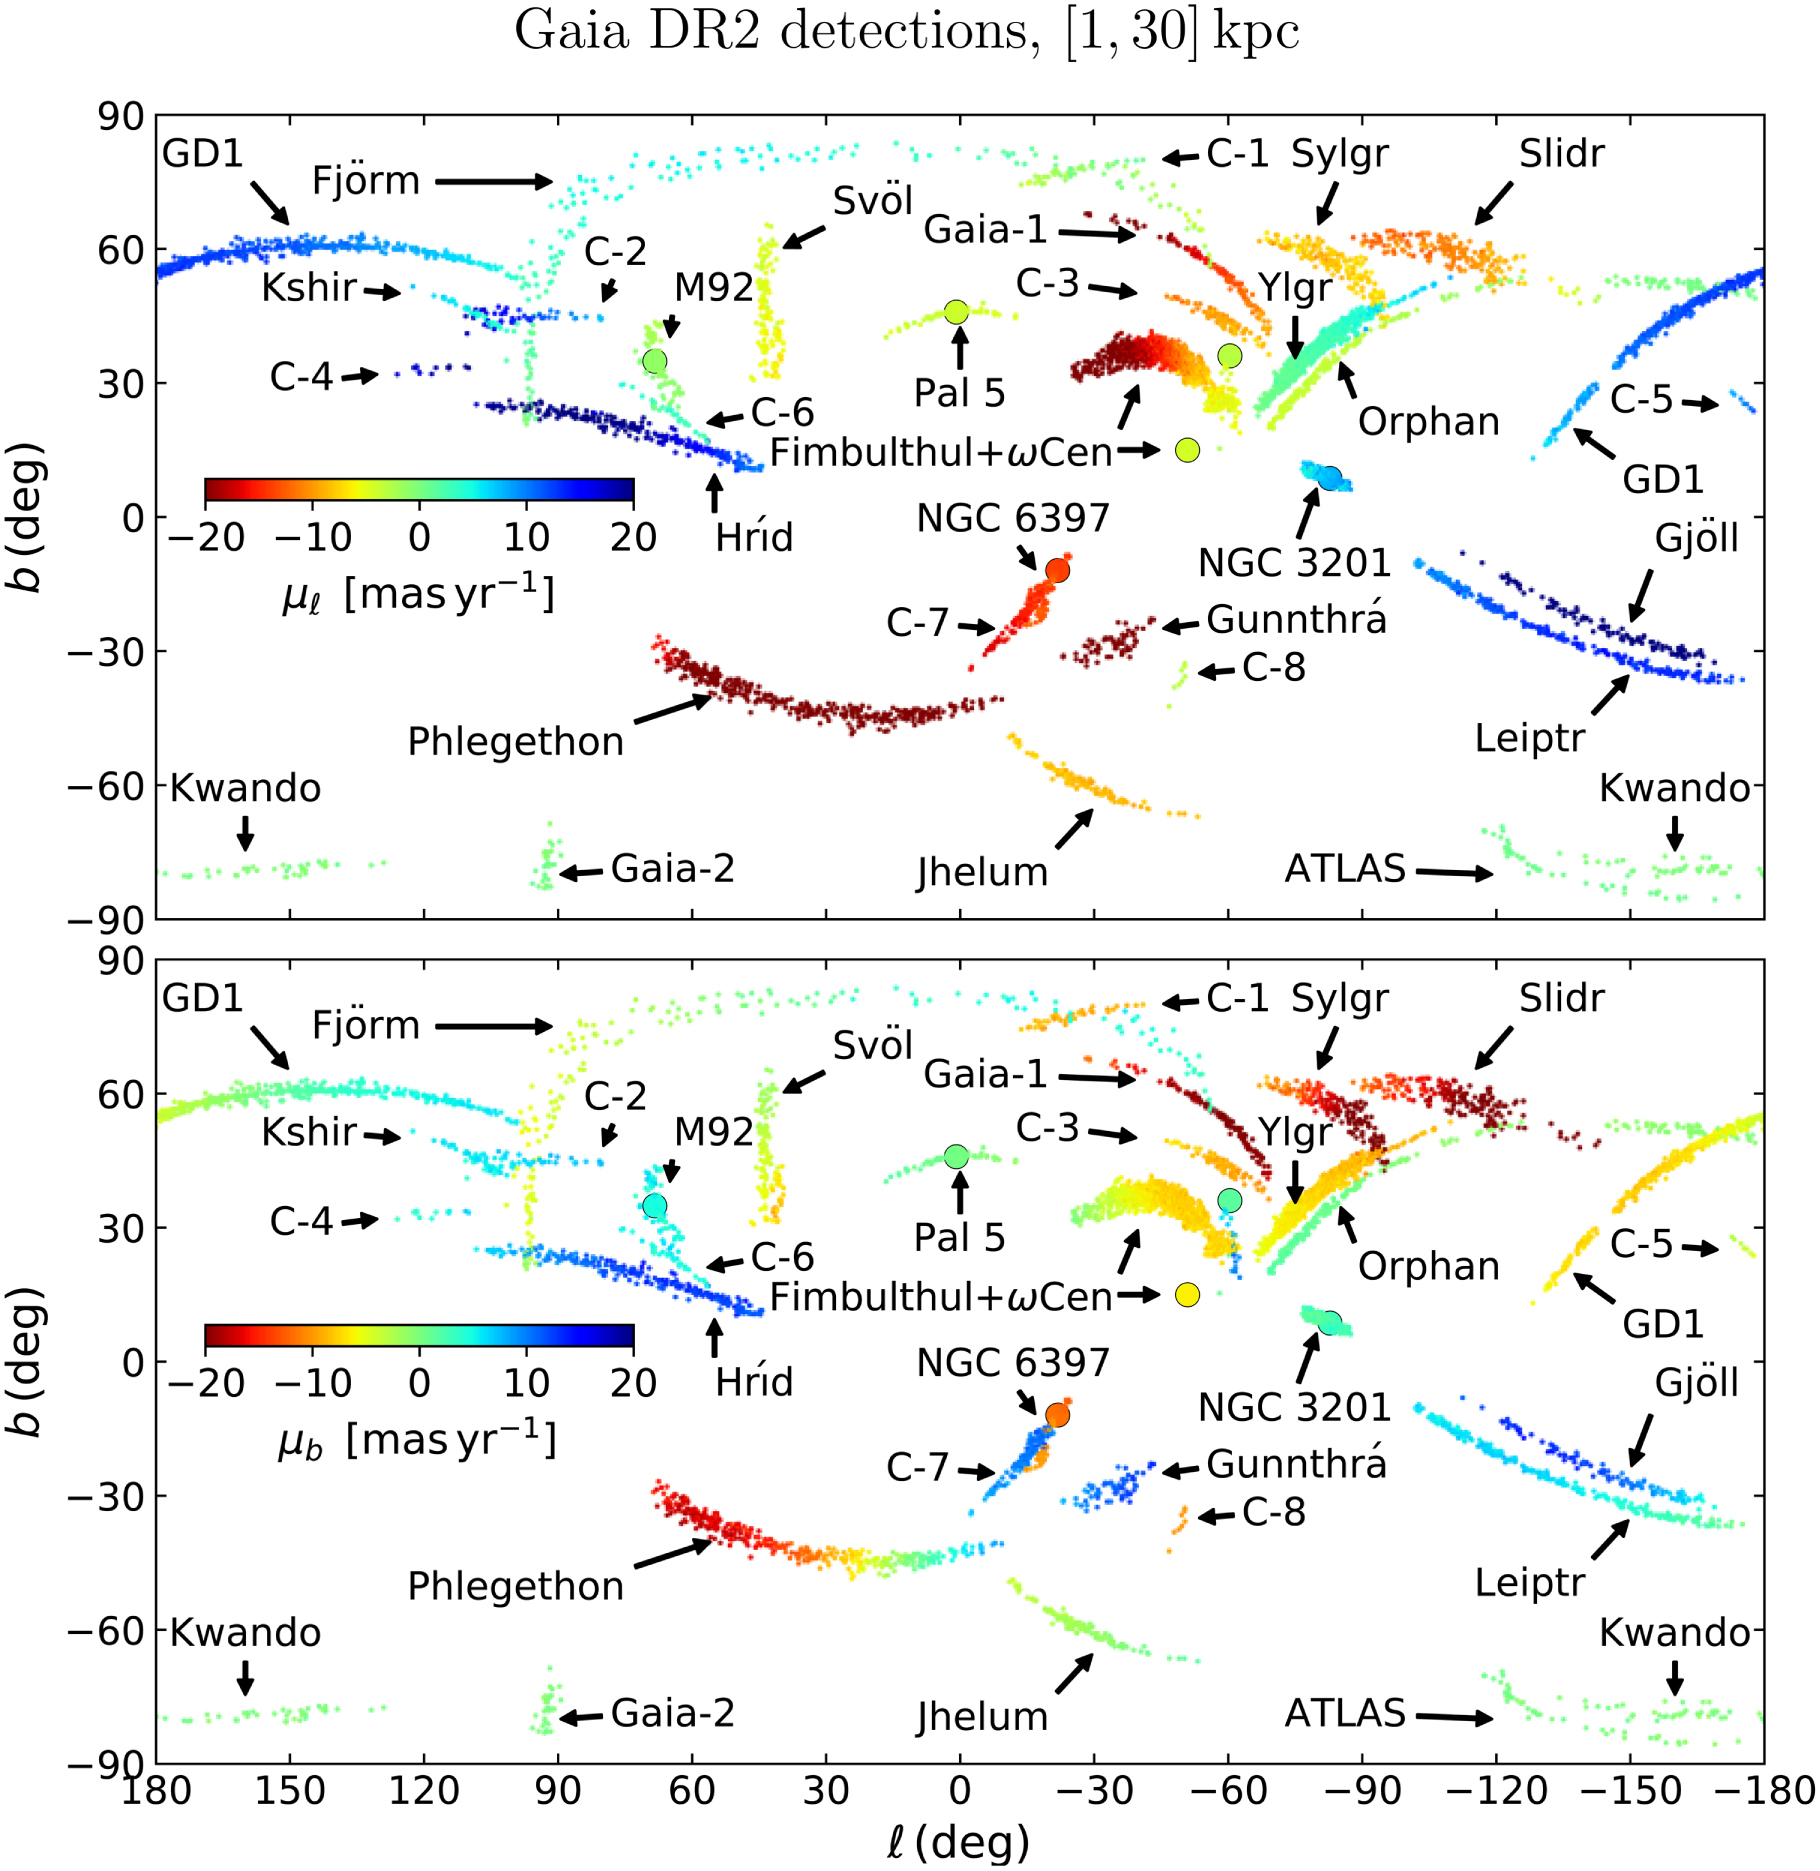
\includegraphics[width=\linewidth]{images/ibata-2021.jpeg}
    \caption{A reported subset of stellar streams within the Milky Way as reported taken from \citet{2021ApJ...914..123I}. These are plotted in Galactic coordinates, in which the celestial sphere is centered about the Sun, 0$^{\circ}$ latitude and longitude points towards the galactic center. These are the streams within 30 kpc of the Sun and were detected using Gaia Data Release 2 \citep{2018A&A...616A...1G}. In the top panel the stars are colored by proper motion in longitude, while the bottom plot shows the stars colored in proper motion in latitude.}
    \label{fig:ibata-2021}
\end{figure}

The fundamental question of where stellar streams originate is well understood. Stellar streams emerge from stars that have liberated themselves from their original stellar systems, courtesy of the forces generated by tidal interactions. Since stellar systems possess are not points and have spatial extent, the region closer to the galactic center of mass, around which they orbit, is subject to a stronger gravitational pull compared to the far side. From the vantage point of the system's center, it appears as though both sides of the extended body are gradually pulled away from the center, culminating in the disintegration of the system and the eventual escape of stars.

This scenario is common for two reasons. The first being that in systems tend to be more massive in the center, always giving rise gravitational fields with gradients, although idealized examples exist such as a uniform infinite sheet of mass. Additionally, self gravitating stellar systems are common. Consequently, stellar streams are ubiquitous across the universe. They materialize when a smaller object is drawn into the gravitational clutches of a larger, more massive counterpart. An illustrative example is the Sagittarius stream, a relic of stars that once belonged to a dwarf galaxy entirely consumed by our Milky Way \citep{2001ApJ...551..294I}. Notably, similar streams may be found in other galaxies, as is the case with the stream encompassing Andromeda (M31) \citep{2001Natur.412...49I}.


Another intriguing source of stellar streams that could account for the observed streams in Fig.\ref{fig:ibata-2021} is none other than globular clusters. Globular clusters are stellar systems characterized by containing between $10^5-10^6$ stars arranged in a spherical distribution. The very first stellar stream known to originate from a globular cluster was Palomar 5, as documented in \citep{2001ApJ...548L.165O}. In such an early study, the discovery of this streams involved identifying an over-density of stars in the vicinity of a globular cluster, followed by a meticulous separation of true stream members from false positives based on color-magnitude data \citep{2003AJ....126.2385O}. Kinematics at the time were not available for large amounts of stars. Interestingly, \citet{2009AJ....137.3378O} revisited the Palomar 5 stream using the Very Large Telescope (VLT) to collect line-of-sight velocity measurements. They were able to confirm that the stars within the stream exhibited matching motion to those within the originating cluster. This methodology is starkly contrasted by those in \citet{2021ApJ...914..123I}, whose search was agnostic. Thanks to the large amounts of data, streams were searched for all over the celestial sphere without targeting specific regions of interest. An interesting consequence of this, is that many of the streams showcased in Fig.\ref{fig:ibata-2021} do not have known progenitors.



Stellar streams serve as invaluable diagnostic tools for investigating various aspects of our Milky Way galaxy. One of the pressing mysteries is the distribution of dark matter. An interesting characteristic of stellar streams is that they generally trace the orbit of the progenitor. By doing so, they can be used to perform inference problems to constrain the gravitational potential of their host galaxy, as highlighted by prior studies such as \citet{2011MNRAS.417..198V}.

Moreover, the utility of stellar streams in probing the gravitational field within which they orbit opens the door to intriguing tests of different cosmological hypotheses. A striking example is the GD-1 stream, a well-known stellar stream that has been employed to scrutinize various scenarios, as documented in \citep{2018ApJ...863L..20P}. Currently, the question of whether globular clusters are formed within dark matter subhalos remains uncertain. A notable investigation by \citet{2019ApJ...881..106M} utilized numerical simulations to demonstrate that the diffuse stellar debris surrounding the GD-1 stream presents compelling evidence of its progenitor cluster forming within a dark matter halo.

Further enriching our understanding, \citep{2021hst..prop16791B} explored the unique `gap' within the GD-1 stream, conducting detailed numerical simulations to constrain the size and mass of the perturbing influence responsible for this feature. Intriguingly, their findings challenge the compatibility of observed gaps with the sizes of dark matter subhalos predicted by the $\Lambda$-CDM cosmological model. These compelling lines of inquiry underscore the multifaceted role of stellar streams in advancing our knowledge of the Milky Way's dynamics and the nature of dark matter.


Unlike the aforementioned studies, my research focuses on examining the collective tidal debris originating from all of the galactic globular clusters, rather than concentrating solely on individual stellar streams. To do so, I leverage a data set of their current known properties that has been refined over the years across multiple studies. In \citet{2021MNRAS.505.5957B}, the authors harnessed a diverse range of data sources, including Gaia DR2 data, the Hubble Space Telescope, and other datasets from the astronomical literature and subsequently determined accurate distances to a multitude of Galactic globular clusters. Furthermore,  \citet{2017MNRAS.464.2174B} use N-Body modeling to construct a staggering 900 simulated globular clusters under various initial conditions, subsequently fitting these models to observed clusters to delve into their internal properties. Building on this foundation, the N-body models were extended to encompass additional galactic globular clusters through the integration of data from the Hubble Space Telescope and Gaia DR2, as detailed in \citet{2020IAUS..351..451H}. This comprehensive work initiated an invaluable online data repository designed to store the kinematic and structural parameters of galactic globular clusters \citep{2021yCat..74781520B}. Initially, this catalog contained orbital and internal properties for 145 globular clusters. With the advent of the third data release from the Gaia mission \citep{2021A&A...650C...3G}, this dataset has expanded its coverage to include a total of 165 globular clusters \citep{2021MNRAS.505.5978V}. These datasets now serve as the foundation for the initial conditions in our simulations, facilitating a more in-depth examination of the tidal debris from galactic globular clusters.



In the subsequent sections of this report, I describe key aspects of our research. I begin by providing a detailed exploration of the physics underlying tidal stripping in Section~\ref{sec:ThePhysics}. Next, in Section~\ref{sec:Computer}, I explain the computational techniques and methodologies employed in our research. Section~\ref{sec:results} offers a comprehensive summary of the results, some of which have already been published in \citep{2023A&A...673A..44F}. Following this, I present preliminary findings from ongoing work, which is currently in the process of being assembled for publication.


